\documentclass[paper.tex]{subfiles}

\begin{document}
    \subsection{Simulation}
    Following results were obtained by running Monte Carlo Simulations of the different process described earlier
    \begin{figure}[ht!]
        \centering
        \subfloat[Poisson Process]{{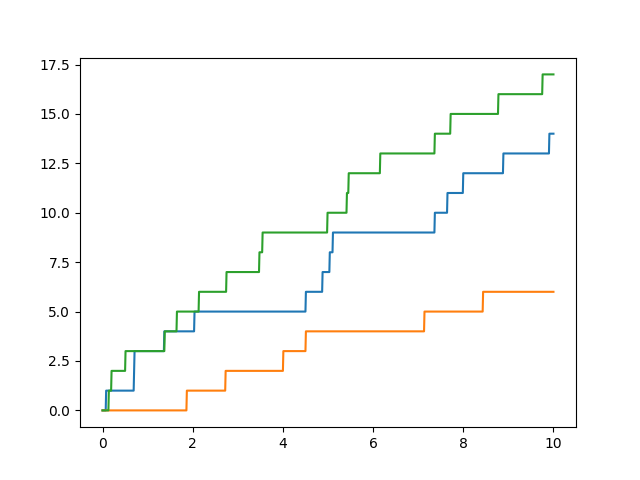
\includegraphics[scale=0.47]{images/poisson-process.png}}}
        \qquad
        \subfloat[Compound Poisson Process]{{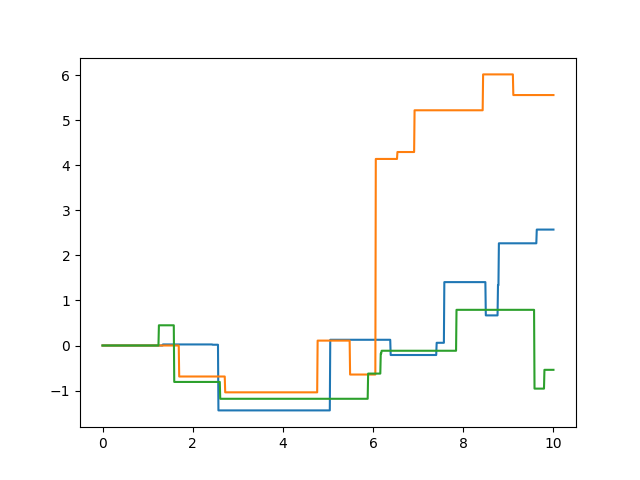
\includegraphics[scale=0.47]{images/compound-poisson-process.png}}}
        \caption{Monte Carlo Simulations of Poisson and Compound Poisson Process.}
        \label{fig: monte-carlo-simulations-1}
    \end{figure}
    \begin{figure}[ht!]
        \centering
        \subfloat[Geometric Brownian Motion]{{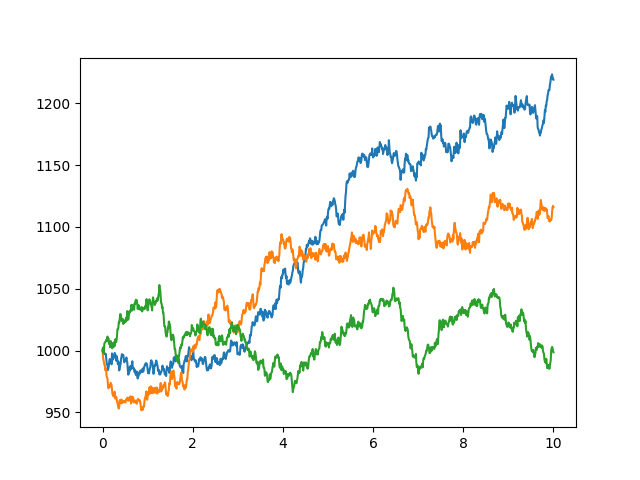
\includegraphics[scale=0.47]{images/geometric-brownian-motion.png}}}
        \qquad
        \subfloat[Jump DIffusion Process]{{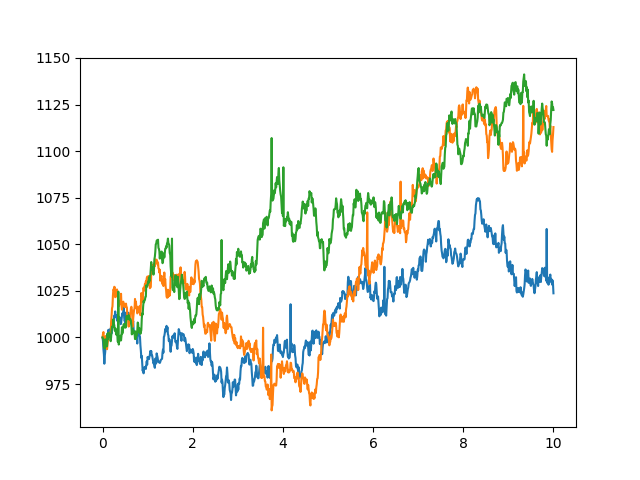
\includegraphics[scale=0.47]{images/jump-process.png}}}
        \caption{Monte Carlo Simulations of Geometric Brownian Motion and Jump Diffusion Process.}
        \label{fig: monte-carlo-simulations-2}
    \end{figure}
    \subsection{Parameter Estimation}
    Model simulations can be run after estimating parameters by using the method (\ref{sec:Estimation of Model Parameters}) mentioned above.
    To calibrate model, first log returns should be found.
    Below are graph of log returns of two stocks `Reliance' and `Zomato'.
    \begin{figure}[ht!]
        \centering
        \subfloat[Reliance log returns]{{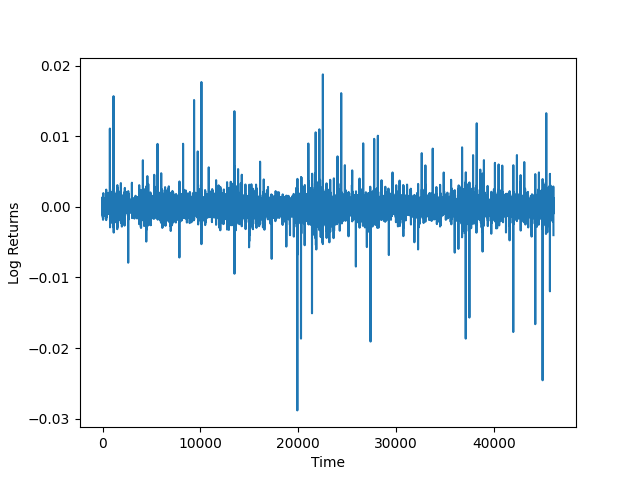
\includegraphics[scale=0.47]{images/reliance-log-returns.png}}}
        \qquad
        \subfloat[Zomato log returns]{{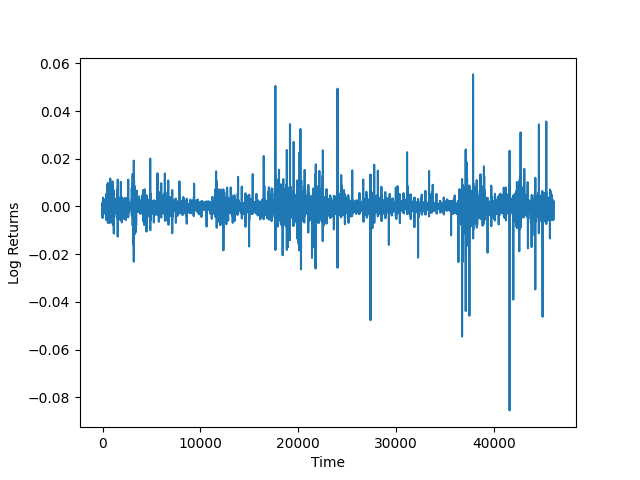
\includegraphics[scale=0.47]{images/zomato-log-returns.png}}}
        \caption{Log Returns calculated at 1 minute frequency from Sep, 2021 to Feb, 2022.}
        \label{fig: log-returns}
    \end{figure}

    Open-Source python package `Scipy' was used to minimize the above described log likelihood function (\ref{eq:log-likelihood-function}).
    Results obtained by applying Maximum Likelihood Estimation method to obtain parameters for some stocks are presented in the following table(\ref{tab: model-parameters}).
    
    \begin{table}[ht!]
        \centering
        \begin{tabular}{|c|c|c|c|c|c|c|}
            \hline
            Stock & $ \lambda $ & $ \mu_{d} $ & $ \sigma_{d} $ & $ \mu_{j} $ & $ \sigma_{j} $ & $ -\text{ln}L $\\
            \hline
            \hline
            Reliance & $1.30 \times 10^{-9} $ & $ 9 \times 10^{-3} $ & 0.131 & 3.358 & 1.265 & -323.90\\
            \hline
            ONGC & $ 1.55 \times 10^{-10} $ & $ 1.36 \times 10^{-2} $ & 0.150 & -$ 7.64 \times 10^{-2} $ & $ 2.87 \times 10^{-3} $ & -291.96\\
            \hline
            Zomato & 0.037 & 0.0149 & 0.177 & -0.0701 & 0.2428 & -236.22\\
            \hline
            Nykaa & 0.480 & $ 0.69 \times 10^{-2} $ & 0.1393 & $ -0.91 \times 10^{-2} $ & 0.150 & -152.48\\
            \hline
        \end{tabular}
        \caption{Estimated parameters by MLE for different stocks for $ \Delta t = $ 1 day}
        \label{tab: model-parameters}
    \end{table}
    
    An interesting obervation from the above Table (\ref{tab: model-parameters}) is that, stocks of large-cap companies such as Reliance and ONGC have very low values of jump parameter $ \lambda $, as compared to newly listed startups such as Zomato and Nykaa.
    It means that on average, there are more jumps in stock price of newly listed companies, which tend to be more volatile than large-cap companies.
    This is inline with the general perception that, public reacts sharply to any new information or news that comes out related to new companies such as Zomato.
    
    According to Black-Scholes,
    
    \begin{equation}
        R_{\Delta T} = \text{ln}\dfrac{S_{T}}{S_{0}} =  ( \mu - \dfrac{\sigma^{2}}{2})\Delta T + \sigma \int_{0}^{T} dW_{t}
        \label{eq: log-returns}
    \end{equation}
    
    Therefore, log returns follows normal distribution with mean and variance as following,
    
    \begin{equation}
        \mathbb{E} \left[ R_{\Delta T} \right] = ( \mu - \dfrac{\sigma^{2}}{2})\Delta T
        \label{eq: log-returns-mean}
    \end{equation}
    \begin{equation}
        \text{Var} \left[ R_{\Delta T} \right] = \sigma^{2}\Delta T
        \label{eq: log-returns-variance}
    \end{equation}
    
    Using the Eq (\ref{eq:log-returns-pdf}) and above equations, the empirical distributions of stock returns can be directly compared with those predicted by BS and MJD model.
    
    \begin{figure}[ht!]
        \centering
        \subfloat[Reliance]{{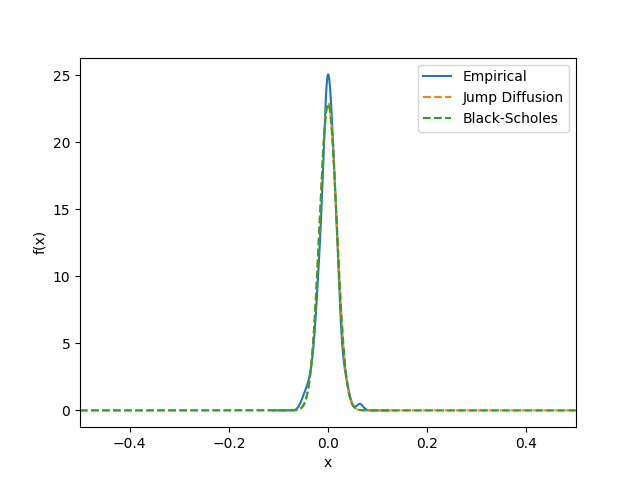
\includegraphics[scale=0.47]{images/reliance-log-returns-distribution.png}}}
        \qquad
        \subfloat[Zomato]{{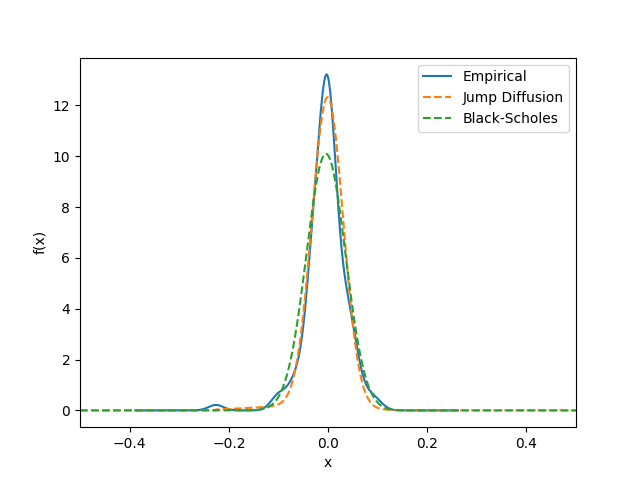
\includegraphics[scale=0.47]{images/zomato-log-returns-distribution.png}}}
        \caption{Daily log returns distribution}
        \label{fig: log-returns-distribution}
    \end{figure}
    
    In the above figures (\ref{fig: log-returns-distribution}), it can be seen that Jump Diffusion model gives a much better approximation to empirical distribution of returns.
\end{document}